\documentclass[9pt,twocolumn]{extarticle}

\usepackage[letterpaper,top=0.58in,bottom=0.62in,left=0.64in,right=0.64in,columnsep=0.23in]{geometry}
\usepackage[T1]{fontenc}
\usepackage{lmodern}
\usepackage{microtype}
\usepackage{booktabs}
\usepackage{graphicx}
\usepackage{balance}
\usepackage{xcolor}
\usepackage[hidelinks]{hyperref}
\usepackage{url}

\hypersetup{
  pdftitle={From Resume Claims to Browser Contracts: A Longitudinal Case Study of LLM-Assisted Visual TDD},
  pdfauthor={An Engineer},
  pdfsubject={A longitudinal case study of LLM-assisted visual TDD},
  pdfkeywords={test-driven development, LLM-assisted engineering, Playwright, visual regression, resume}
}

\definecolor{accent}{HTML}{087A55}
\setlength{\parindent}{0.9em}
\setlength{\parskip}{0pt}
\setlength{\columnsep}{0.23in}
\renewcommand{\arraystretch}{1.04}
\setcounter{dbltopnumber}{1}
\renewcommand{\dbltopfraction}{0.72}
\urlstyle{same}

\makeatletter
\renewcommand{\section}{\@startsection{section}{1}{0pt}%
  {0.8ex plus 0.25ex minus 0.15ex}{0.3ex}%
  {\normalfont\large\bfseries\color{accent}}}
\renewcommand{\subsection}{\@startsection{subsection}{2}{0pt}%
  {0.55ex plus 0.2ex minus 0.1ex}{0.15ex}%
  {\normalfont\normalsize\bfseries}}
\makeatother

\title{\vspace{-1.55em}\textbf{From R\'esum\'e Claims to Browser Contracts:}\\[-0.1em]
\large A Longitudinal Case Study of LLM-Assisted Visual TDD}
\author{An Engineer\\[-0.2em]
\small Identifying details and page text are withheld}
\date{}

\begin{document}
\maketitle
\vspace{-1.55em}

\begin{abstract}
Modernizing a r\'esum\'e website is usually described as a framework migration. Through a single-artifact longitudinal case study, we examine a different formulation: the page is a public claim interface, and its redesign is governed by browser contracts. We compare a still-deployed legacy artifact with its replacement using Playwright at matched desktop and mobile viewports, inspect an 18-commit development trace, and independently rerun overflow, overlap, typography, geometry, semantic, and pixel checks. The redesign reduced above-fold words from 262 to 91 on desktop and from 118 to 57 on mobile, eliminated 27 and 23 sub-13-pixel text elements, restored all four structural landmarks, and reduced alignment near-misses from 32 to 4 and from 27 to 1. The suite grew from no browser tests to 20 test declarations (21 executed cases) and two visual baselines. We argue that the practical outcome is not only safer front-end code: engineers gain a controlled LLM workflow, while recruiters receive a more stable, scannable, and verifiable evidence surface. The study offers a reproducible pattern for turning subjective redesign into bounded, test-driven iteration.
\end{abstract}

\textbf{Keywords:} visual TDD, Playwright, LLM-assisted engineering, r\'esum\'e, visual regression

\section{Introduction}
A public r\'esum\'e is read by people, crawlers, assistive technologies, and deployment systems. Its correctness therefore exceeds valid markup. A claim can be accurate yet effectively absent below the fold; a polished desktop can fail on mobile; a detailed route can leak into search; a harmless color edit can leave a sticky header visibly detached from its section. These failures are observable, but conventional modernization work rarely makes them explicit.

The case studied here began with generated output from a legacy site generator. Its source model was missing, facts and layout were coupled, and publication had no browser gate. An LLM accelerated reconstruction and redesign, but it also increased the rate at which broad, plausible changes could be proposed. The response was to treat tests as the control surface: the human states an intended reader outcome, the LLM makes the smallest relevant edit, and a browser decides whether the observable contract holds. We call the executable specification a \emph{contract}; its assertions, traces, measurements, screenshots, and deployed responses are the resulting \emph{evidence}.

We ask three questions. \textbf{RQ1:} Which visual and semantic changes are measurable between the live legacy and modern artifacts? \textbf{RQ2:} How did browser contracts evolve across the commit sequence rather than appearing only after implementation? \textbf{RQ3:} What value does this testing model provide beyond development, particularly to engineers maintaining their public record and recruiters evaluating it?

Our contribution is a paired-artifact protocol, a longitudinal account of LLM-assisted visual TDD, and a stakeholder interpretation of tests as durable evidence rather than release-time ceremony.

Figure~\ref{fig:method} presents the intervention and measurement loops; Fig.~\ref{fig:xray} the paired visual x-ray; Fig.~\ref{fig:commits} the commit trajectory; and Fig.~\ref{fig:contracts} representative browser contracts.

\begin{figure*}[t]
\centering
\begin{minipage}[t]{0.42\textwidth}
  \centering
  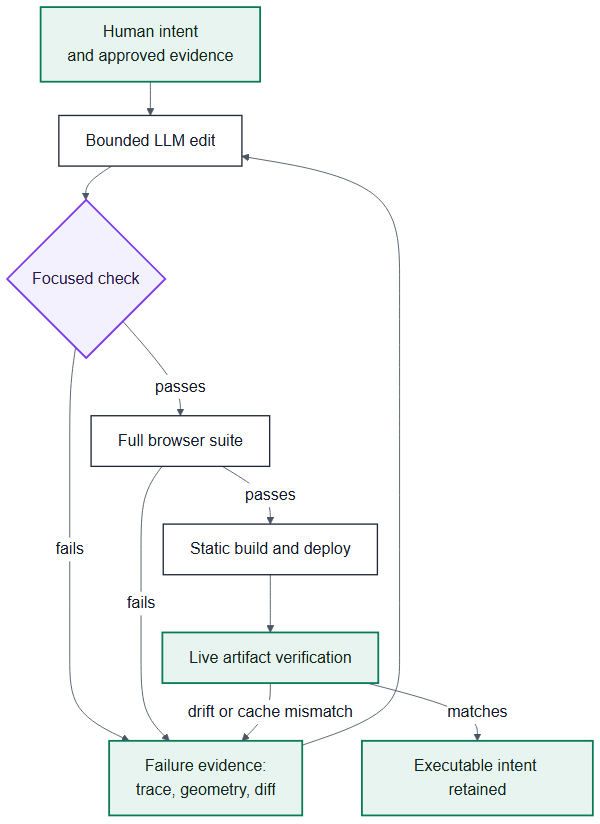
\includegraphics[height=2.28in]{figures/llm-tdd-loop.png}
  \par\footnotesize (a) Bounded LLM intervention loop
\end{minipage}\hfill
\begin{minipage}[t]{0.54\textwidth}
  \centering
  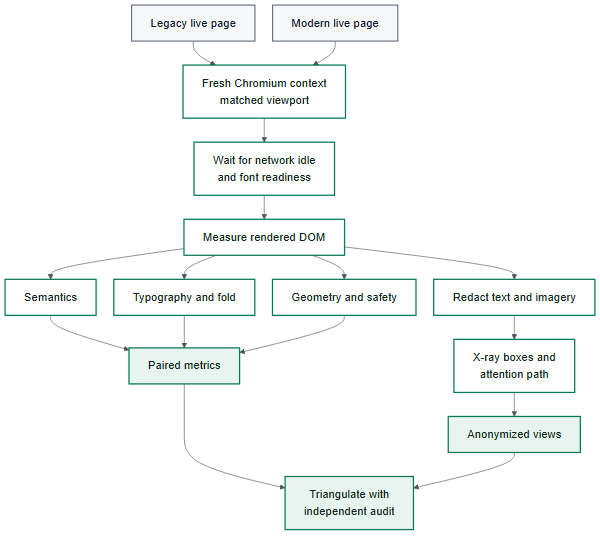
\includegraphics[height=2.28in]{figures/visual-study-protocol.png}
  \par\footnotesize (b) Matched visual-study protocol
\end{minipage}
\caption{Method flow. Failures return concrete browser evidence to the next edit; visual comparison uses isolated contexts, matched viewports, pre-redaction measurements, and an independent audit.}
\label{fig:method}
\vspace{-0.5em}
\end{figure*}

\begin{figure*}[t]
\centering
\begin{minipage}[t]{0.485\textwidth}
  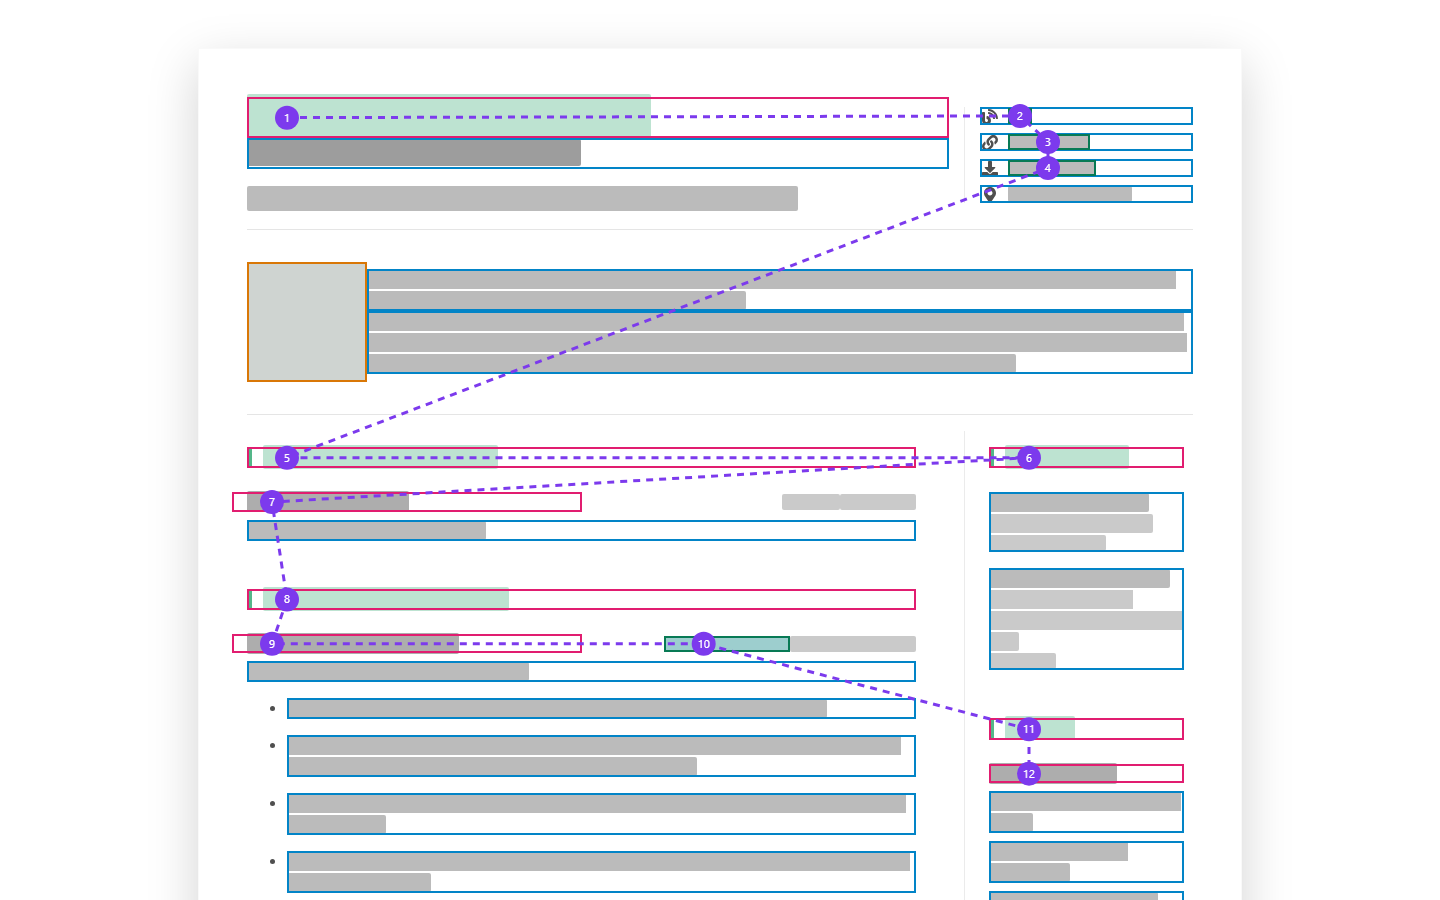
\includegraphics[width=\linewidth]{figures/legacy-desktop-xray.png}
  \centering\footnotesize (a) Legacy first viewport
\end{minipage}\hfill
\begin{minipage}[t]{0.485\textwidth}
  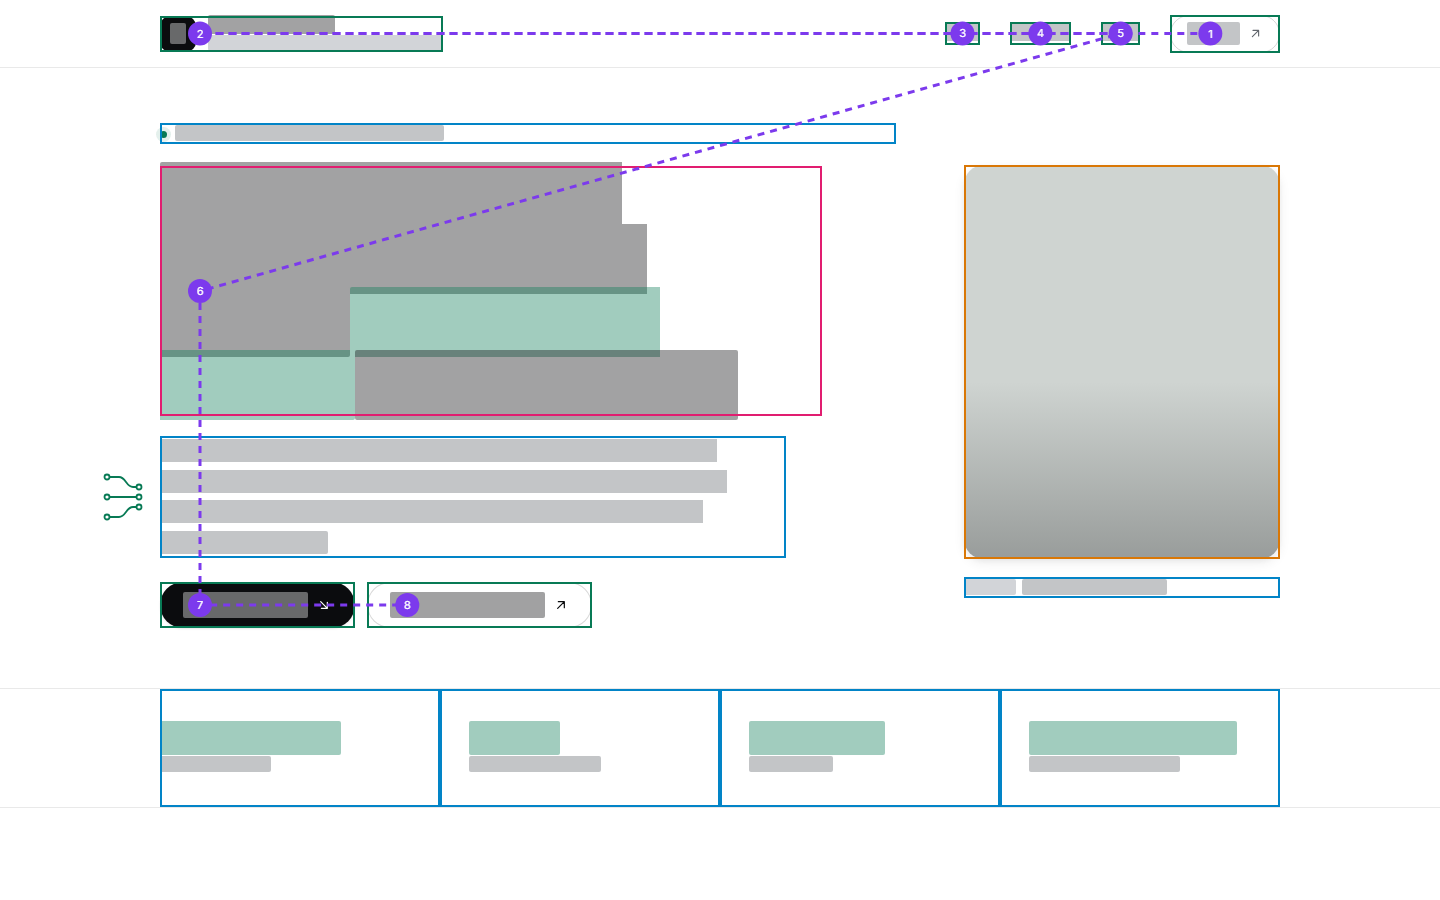
\includegraphics[width=\linewidth]{figures/modern-desktop-xray.png}
  \centering\footnotesize (b) Modern first viewport
\end{minipage}
\caption{Matched Playwright x-rays at $1440\!\times\!900$. Magenta, blue, green, and orange boxes denote headings, prose/lists, actions, and media; the dashed path orders first-fold attention anchors. Text is replaced after measurement and images become neutral blocks. The legacy view exposes competing columns and cross-column jumps; the replacement establishes one dominant thesis before evidence.}
\label{fig:xray}
\vspace{-0.5em}
\end{figure*}

\begin{figure*}[t]
\centering
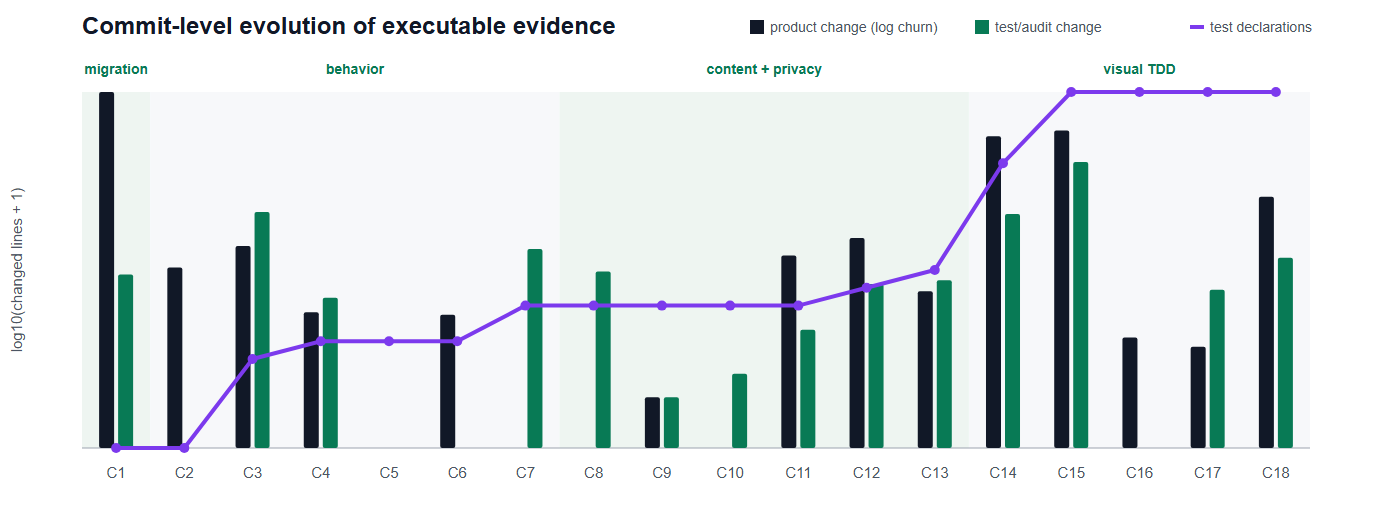
\includegraphics[width=0.9\textwidth]{figures/commit-trajectory.png}
\caption{Commit-level trace. Bars show log-scaled changed lines in product code and test/audit infrastructure; the line shows cumulative browser-test declarations. Tests precede and accompany the largest visual interventions rather than being appended at release time.}
\label{fig:commits}
\vspace{-0.7em}
\end{figure*}

\begin{figure*}[t]
\centering
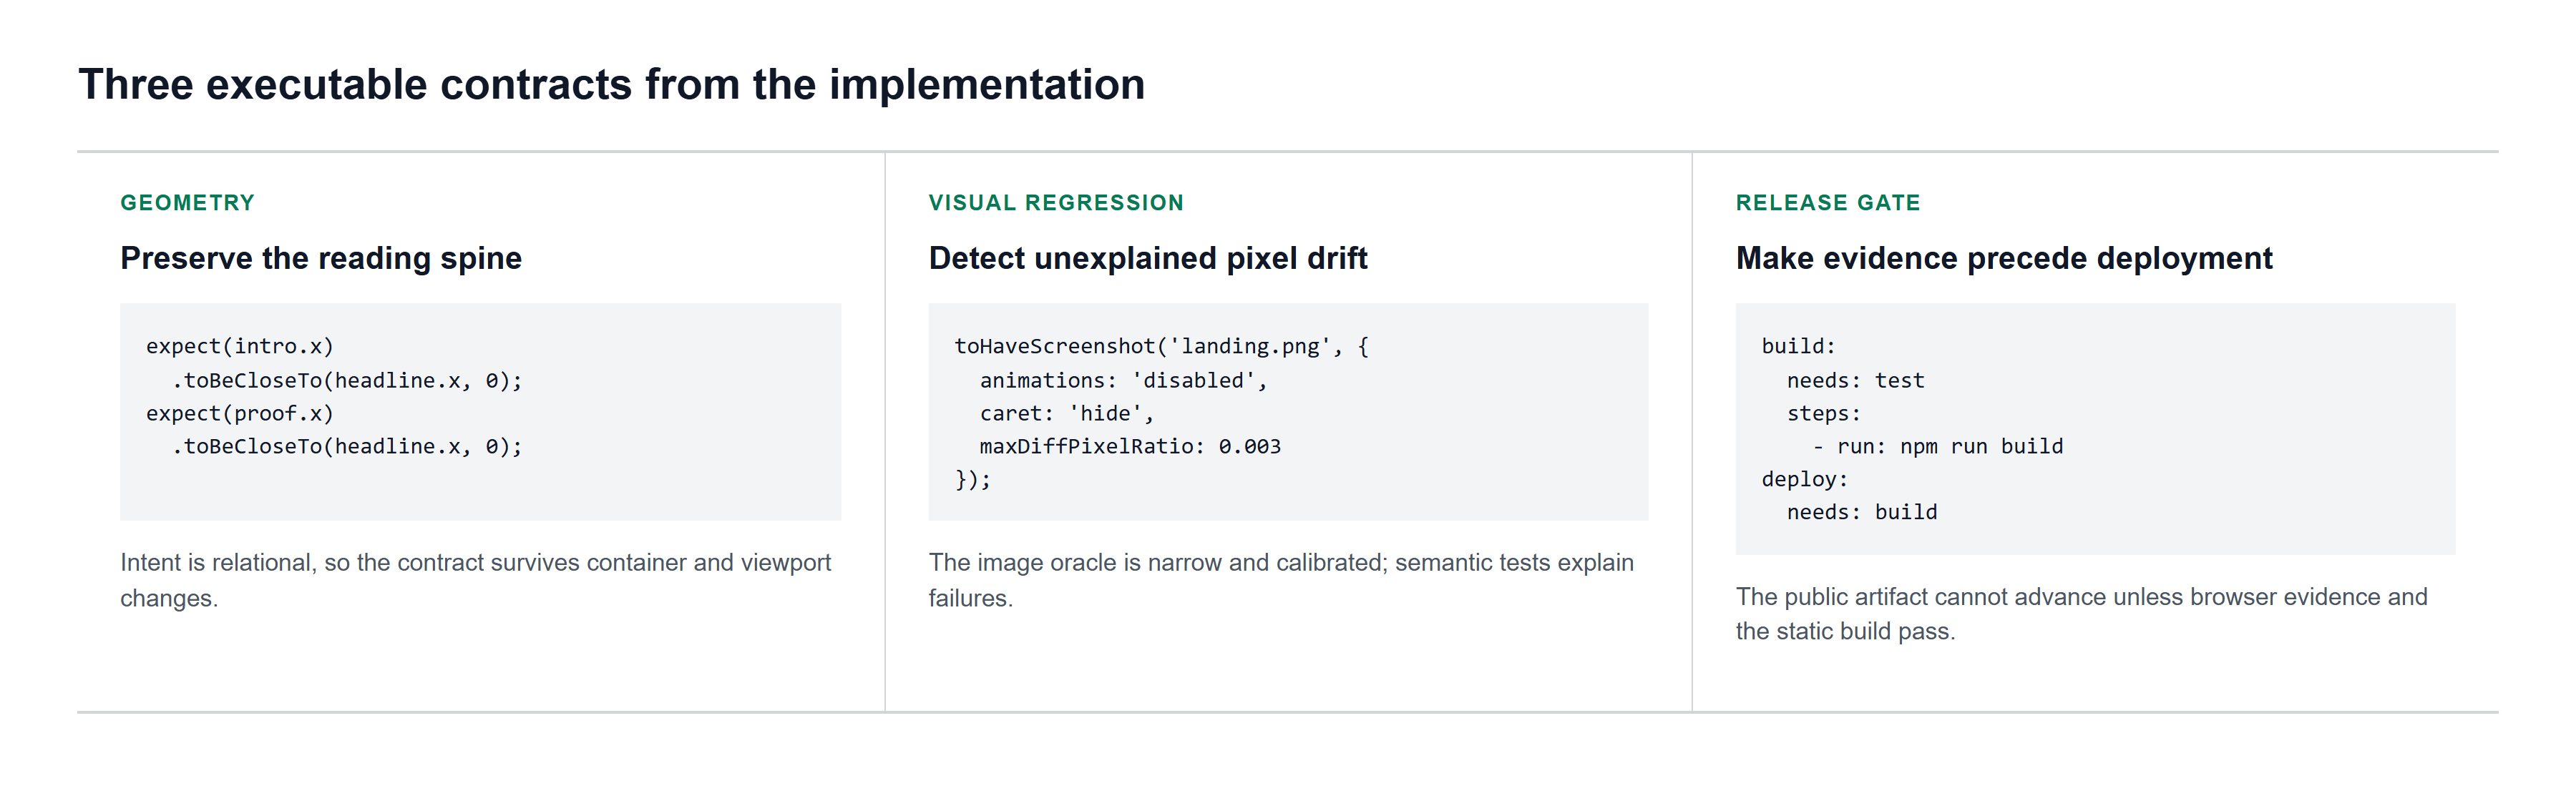
\includegraphics[width=\textwidth]{figures/executable-contracts.png}
\caption{Abridged implementation excerpts. Geometry preserves a relational reading spine, raster comparison detects unexplained drift, and the release graph prevents publication before browser tests and the static build pass.}
\label{fig:contracts}
\vspace{-0.6em}
\end{figure*}

\section{Related Work}
TDD treats a failing test as a statement of intended behavior and uses short implementation cycles to make that statement true~\cite{beck2002}. Visual interface work complicates the idea of an oracle: exact pixels are observable, but they are not equivalent to usability. Industrial visual-GUI testing therefore combines image comparison with structural checks and human interpretation~\cite{alegroth2017}. Our method follows that division. Pixel snapshots signal unexplained change; semantic and geometric assertions explain why a change matters.

AutoMan generates a verified implementation baseline from TLA+-style specifications, then permits selective manual optimization under refinement proofs~\cite{automan2025}. We adopt its division of effort, not its guarantee: TLA+ model-checks the publication protocol, while Astro and CSS are manually optimized and checked at observable boundaries with Playwright. No code generator or machine-checked implementation refinement is claimed.

Studies of code-generating assistants describe programmers alternating between acceleration and verification. Grounded interaction emerges when developers inspect, steer, and repair generated code rather than accepting whole solutions~\cite{barke2023}; controlled evidence also suggests productivity gains for suitable tasks~\cite{peng2023}. This case contributes a visual counterpart: the model can search CSS, propose hierarchy, and author assertions, but approved facts and browser observations remain external constraints.

Recent hiring-focused preprints make the safety boundary more concrete. LLM-assisted application materials can create strategic advantages and distort downstream selection~\cite{cohen2025}; automated screening therefore demands counterfactual, group, and merit-aware evaluation rather than one reassuring aggregate~\cite{yashwant2026}. We do not score candidates or claim fairness effects. These studies instead motivate our refusal to treat visual polish as evidence about hiring outcomes.

Three complementary systems inform the control structure. Takano finds prompt guardrails helpful but insufficient against fabricated resume claims, with human checkpoints strongest on severe identity failures~\cite{takano2026}. Bishop et al. show how typed intermediate state and retained provenance can reduce misinformation while carefully labeling recipient benefit as an artifact-level estimate~\cite{bishop2026}. Attune compiles human steering into inspectable constraints rather than relying on natural-language intent alone~\cite{chopra2026}. Our structured resume data, explicit claim approval, and executable browser contracts apply the same broad reliability principles to public-page authoring without adopting those systems' tasks or evaluation claims.

The reader-facing motivation connects to information foraging. People follow cues that promise useful information relative to the cost of reaching it~\cite{pirolli1999}. We do not infer gaze from the DOM. Instead, fold density, hierarchy, landmarks, and alignment operationalize prerequisites for low-cost navigation, while WCAG provides normative guidance for semantic and perceptual access~\cite{wcag22}. The resulting claims concern observable presentation and process reliability, not recruiter cognition itself.

\section{Study Design}
\subsection{Artifacts and privacy}
The study uses two public deployments that encode the same professional history: a legacy generated page and the final static replacement. URLs are supplied to the reproduction script through environment variables and are not stored in the paper. Metrics are computed before anonymization. For figures, Playwright replaces every text node with an opaque block of identical layout extent and replaces images with neutral blocks; names, employers, locations, contact details, and facial structure are therefore absent. The study reports aggregate geometry and test counts only.

We analyze 18 commits from the framework migration through the final visual refinement. Each commit is represented as $C_1\ldots C_{18}$, preserving order without exposing repository identifiers. Diff paths are grouped into product code, structured content, test/audit infrastructure, and other files. We count declared browser-test sites at each revision and separately report executed cases where parameterization creates more than one case.

\subsection{Matched Playwright protocol}
Fresh Chromium contexts load each deployment at $1440\!\times\!900$ and $390\!\times\!844$ with reduced motion. After network idle and font readiness, the script inspects only rendered elements. \emph{Fold words} count words in direct visible text nodes intersecting the first viewport. \emph{Hierarchy ratio} is the largest heading size divided by the median visible text size. \emph{Small text} counts nodes below 13 pixels. \emph{Landmark completeness} records the presence of \texttt{header}, \texttt{nav}, \texttt{main}, and \texttt{footer}. An \emph{alignment near-miss} occurs when a semantic element's left edge is 2--12 pixels from a recurring edge shared by at least three elements.

The x-ray draws bounding boxes around headings, prose, actions, and media, then connects the first twelve heading/action anchors in visual order. A second implementation independently scrolls the full document and checks undersized text, horizontal overflow, and pairwise text intersections. This triangulation matters: a page can pass overflow checks while still presenting weak hierarchy or a noisy scan path. Screenshot assertions then guard stable high-value regions against later pixel drift~\cite{playwright,alegroth2017}.

Figure~\ref{fig:method} separates the two loops that are often conflated in accounts of LLM-assisted development. Panel (a) is the intervention loop: model output advances only when focused and full-suite evidence passes, and deployment remains observable. Panel (b) is the measurement loop: both artifacts receive the same browser treatment before their metrics and anonymized views are triangulated. The diagrams are maintained as Mermaid source and pre-rendered to static PNG, keeping the paper build independent of browser JavaScript.

\subsection{Oracle hierarchy and formal core}
The method orders checks by explanatory power and cost. Structured-data validation is the earliest oracle: it rejects malformed URLs, impossible field combinations, and unknown content before rendering. Rendered-string and accessibility-tree assertions then check whether approved claims appear under the intended headings and landmarks. These tests are narrow enough to identify the broken contract, yet they execute in the same browser as the final page.

Post-study hardening adds a finite TLA+ state machine for environment, request, content provenance, indexing, validation, build, and deployment state. TLC exhaustively checks 30 reachable states to depth 6 against five invariants. Three mutation models deliberately introduce a private-overlay leak, an indexed preview, and deployment without validation; TLC rejects each with a two-state counterexample. These results validate the abstract protocol and the sensitivity of its invariants, not the full UI implementation.

\subsection{Score-guided iteration within a verified envelope}
The formal core also bounds a second question: given a legible page, which design-token settings should the next iteration adopt? We model four tokens---body size, heading size, fold budget, and section spacing---as a second finite TLA+ machine, \texttt{VisualVariant}. Its admissibility invariant encodes the legibility and layout constraints recovered from the study (body no smaller than 13\,px, heading within a bounded range, fold budget and spacing within measured limits). TLC enumerates the full token grid of 945 states and certifies that exactly 200 satisfy admissibility; a mutation that shrinks the body below 13\,px is rejected with a counterexample. The 200-state feasible region is the search space; the other 745 combinations are pruned \emph{before} any tuning, because they are formally unsafe rather than merely undesirable.

Within that region we define a \emph{score}: a declared weighted objective in $[0,1]$ that measures how close a variant sits to the target values recovered from the modern artifact (a larger body, a heading near 38\,px, a fold budget near 80 words, and generous spacing), with weights favoring reading-spine hierarchy over cosmetic spacing. The score is an explicit engineering objective over measurable tokens; it is emphatically not a model of perceived beauty. Its role is to make ``which variant next'' reproducible and auditable rather than a matter of taste.

Two searches optimize the score over the verified region. Exhaustive search establishes the true optimum; a guarded greedy search tests whether the region is smooth enough to climb without leaving it. Both reach the same optimum, raising the seed score from 0.858 to 0.970 (a 13.1\% gain) in two steps, and the guarded search visits zero inadmissible states. Crucially, the implementation's independent enumeration of the feasible region agrees exactly with TLC's 200 reachable states; a divergence between the code and the model would fail the check. This is the core contribution of the formal layer to visual work: verification does not choose the design, it \emph{fences the space of designs the optimizer may propose}, so no score-improving step can produce an illegible or unpublishable page. The optimizer emits a human-in-the-loop recommendation; it never writes stylesheet values directly.

Geometry is relational rather than absolute wherever possible. An assertion that an introduction and proof label share the headline's x-coordinate survives changes in container width; a minimum font-size assertion survives copy edits. Raster snapshots are reserved for high-value regions because they detect residual changes that are difficult to enumerate, but their failure is diagnostic evidence, not an automatic verdict. Animations and carets are disabled, fonts are awaited, and baselines are calibrated to a named browser and operating system.

Finally, publication checks cross the repository boundary. The suite builds and serves the static output, requests crawler resources, inspects indexing directives, and verifies alternate public views. After deployment, the same reasoning distinguishes a source defect from workflow failure or edge-cache staleness. This layered oracle prevents a common category error: a unit-level pass cannot establish that the artifact a recruiter receives is the artifact the author tested.

Figure~\ref{fig:contracts} shows how these layers appear in code. Each excerpt is intentionally small: one relation protects the reading spine, one calibrated screenshot protects residual appearance, and two dependency edges protect publication order. The value lies in composing narrow contracts, not in replacing judgment with a large test framework.

\section{Results}
\subsection{RQ1: Visual and semantic change}
Table~\ref{tab:results} reports the paired observations. The desktop fold contains 65.3\% fewer words after modernization; mobile contains 51.7\% fewer. This is not content deletion: document length increases from 4.18 to 7.83 desktop viewports and from 9.71 to 12.73 mobile viewports because evidence is progressively disclosed below a focused opening. The result is a change in ordering, not simply brevity.

\begin{table}[ht]
\centering
\caption{Matched live-page measurements. D=desktop, M=mobile.}
\label{tab:results}
\footnotesize
\begin{tabular}{lrrrr}
\toprule
& \multicolumn{2}{c}{Legacy} & \multicolumn{2}{c}{Modern} \\
\cmidrule(lr){2-3}\cmidrule(lr){4-5}
\textbf{Measure} & \textbf{D} & \textbf{M} & \textbf{D} & \textbf{M} \\
\midrule
Fold words & 262 & 118 & 91 & 57 \\
Hierarchy ratio & 2.46 & 2.46 & 3.87 & 2.80 \\
Text $<13$ px & 27 & 23 & 0 & 0 \\
Landmarks (/4) & 1 & 1 & 4 & 4 \\
Alignment near-misses & 32 & 27 & 4 & 1 \\
Horizontal overflow & 0 & 0 & 0 & 0 \\
Significant overlap & 0 & 0 & 0 & 0 \\
\bottomrule
\end{tabular}
\end{table}

The hierarchy ratio rises 57.3\% on desktop, consistent with the single dominant region in Fig.~\ref{fig:xray}. Near-misses fall 87.5\% on desktop and 96.3\% on mobile. Yet both artifacts record zero overflow and overlap. This negative result is informative: responsive safety is necessary but does not measure rhetorical clarity. Semantic structure changes from one of four landmarks to four of four, and an explicit \texttt{h1} replaces a page with no level-one heading. The independent audit reproduces the zero-overflow result and the 27/23 versus 0/0 small-text contrast.

The disagreement among metrics is itself a result. A binary overflow check would rate the artifacts equally, while typography, hierarchy, semantics, and alignment expose different failure families. This echoes multi-family auditing in candidate-ranking research, where score, rank, and shortlist measures can disagree~\cite{yashwant2026}. Our measures are descriptive rather than inferential, but reporting them separately prevents a composite ``quality score'' from concealing the reason a page changed.

\subsection{RQ2: Evidence accumulated with the design}
Figure~\ref{fig:commits} reconstructs the engineering sequence. The initial migration ($C_1$) established structured source and static deployment. Browser tests appeared at $C_3$, before later analytics, privacy, content, and visual interventions. The suite reached eight test declarations by $C_7$, ten by $C_{13}$, and twenty by $C_{15}$; the final studied revision executes 21 cases because one declaration is parameterized. Pixel baselines first appear at $C_{15}$.

Two episodes illustrate the control loop. A perceived alignment defect became an equality test over the x-coordinates of the headline, introduction, and first proof item. A gray ribbon over a dark section became two assertions: the sticky header must equal the section's computed background color and its lower edge must meet the section within one pixel. In each case the LLM searched and edited; Playwright supplied the falsification boundary. This resembles grounded interaction with code-generation tools, where useful acceleration depends on feedback and developer control~\cite{barke2023,peng2023}.

\section{RQ3: Practical Implications}
\textbf{For engineers, tests become a memory of intent.} A schema prevents unsupported fields from entering the public model. Semantic tests preserve the thesis, proof labels, heading order, crawler output, and indexing policy. Geometry tests retain design intent without freezing a CSS implementation, while a small number of calibrated screenshots detect unexplained drift. Deployment tests extend the boundary to the live artifact: source revision, generated output, and cache behavior can be distinguished when a page appears stale. The LLM is consequently useful as a fast search-and-synthesis partner, but not as the source of truth. Claims require human provenance; design proposals require visual review; every accepted change leaves an executable reason behind it.

\textbf{For recruiters, the benefit is lower verification cost.} The modern fold presents one positioning claim, then explicit evidence, before chronology. Larger type and fewer alignment near-misses reduce competition for attention; semantic landmarks and a real heading hierarchy improve navigation for assistive tools and parsers under WCAG-informed practice~\cite{wcag22}. Tests also protect practical trust signals: dates remain attached to roles, links resolve, public and detailed variants retain their intended disclosure policy, and mobile readers receive the same evidence order. These checks do not certify that a career claim is true, nor should they automate candidate ranking. They ensure that approved evidence is legible, stable, and consistently published.

That boundary is consequential. Work on strategic LLM manipulation and counterfactual bias shows that application assistance and automated screening interact with unequal access and protected signals~\cite{cohen2025,yashwant2026}. A well-tested candidate page must not be mistaken for a fair hiring system. Its legitimate contribution is narrower: reducing accidental presentation variance while preserving the candidate's approved account.

At screening time, the useful unit is not an aesthetic score but \emph{time to evidence}. A reader is implicitly asking what the candidate builds, at what demonstrated scale, and where the supporting record appears. Information-foraging theory predicts that clear cues reduce the cost of deciding where to look next~\cite{pirolli1999}. Visual TDD cannot measure cognition directly, but it can preserve its preconditions: one dominant opening claim, evidence within the initial viewport, stable label--value relationships, and the same order on a narrow screen. This yields a falsifiable follow-up study: compared with the legacy page, recruiters should locate a target capability and its supporting example faster and with higher recall.

The same argument extends beyond hiring. A public profile is consumed by search previews, social cards, accessibility trees, crawlers, and archival caches. Tests make those secondary representations reviewable alongside the visible page. They also expose disagreement between source and deployment: a passing local screenshot does not explain a stale public response, whereas a chain from commit, build artifact, response metadata, and cache-busted render does. In that sense, the suite functions as provenance for presentation.

This distinction moves testing beyond developers. The author uses failures as editorial prompts; a designer receives measurable constraints; a recruiter encounters fewer presentation defects; and future maintainers inherit a specification of what the page is trying to communicate. The test suite is therefore part of the public document's governance, even though readers never see it.

\section{Reproducibility and Release}
The companion artifact keeps measurement separate from publication. Playwright scripts accept page locations and revision bounds at runtime, emit aggregate JSON, redact the DOM, and generate the x-rays and commit trace. Mermaid sources and a browser renderer generate Fig.~\ref{fig:method}. Every reported number and view therefore has a generation path, while the manuscript stores no identifying endpoint.

\textbf{AI-use disclosure.} GitHub Copilot assisted repository search, implementation and CSS edits, test drafting, diagnostics, and prose revision. The author approved every professional claim, selected the questions and metrics, interpreted the evidence, verified citations and diffs, and accepted the manuscript. No model established claim truth or conclusion validity.

\textbf{Artifact availability.} The public release includes measurement scripts, anonymized metrics, Mermaid sources, figures, and a minimal arXiv archive; raw identifying captures are excluded. Double-blind review requires a separate anonymized repository with rewritten history. The public repository and live page suit only arXiv or single-blind review.

The arXiv package contains top-level PDFLaTeX source and static PNGs through \texttt{graphicx}; it excludes JavaScript, image conversion, compiler products, and the generated PDF. A local page-by-page review checks figure semantics that successful TeX processing cannot establish.

\section{Threats to Validity}
This single-artifact longitudinal case study is not a causal evaluation of recruiter behavior. The author is the artifact owner, intervention designer, and evaluator, which may influence metrics, stopping, and interpretation. Scripts, commit history, and an independent audit make choices inspectable but do not remove this reflexivity. DOM attention paths are proxies, not eye tracking; reader performance is motivation, not the estimand~\cite{bishop2026}. Content length also changes, screenshots are platform-sensitive, and alignment and font thresholds are operational definitions. Tests preserve approved claims but cannot establish their truth.

\section{Conclusion}
The modernization was not successful because one generator replaced another. It became defensible when an LLM-assisted sequence added browser contracts and retained their evidence alongside the interface. Across live-page measurements and 18 commits, the resulting system improved first-fold focus, hierarchy, semantics, text legibility, and alignment while retaining explicit checks for responsive safety and disclosure. For engineers, visual TDD constrains rapid generation. For recruiters, it lowers friction between a claim and the evidence needed to assess it. A public r\'esum\'e can be treated not as a finished page, but as a small, continuously verified information system.

\begin{thebibliography}{9}
\fontsize{6.5}{7.2}\selectfont
\setlength{\itemsep}{0pt}
\setlength{\parsep}{0pt}
\bibitem{beck2002} K. Beck, \emph{Test Driven Development: By Example}. Addison-Wesley, 2002.
\bibitem{playwright} Microsoft, ``Playwright: Visual comparisons and assertions,'' 2026. [Online]. Available: \url{https://playwright.dev/docs/test-snapshots}
\bibitem{alegroth2017} E. Al\'egroth, R. Feldt, and L. Ryrholm, ``Visual GUI testing in practice: Challenges, problems and limitations,'' \emph{Empirical Software Engineering}, vol. 22, 2017.
\bibitem{barke2023} S. Barke, M. B. James, and N. Polikarpova, ``Grounded Copilot: How programmers interact with code-generating models,'' \emph{Proc. ACM Program. Lang.}, vol. 7, OOPSLA1, 2023.
\bibitem{peng2023} S. Peng, E. Kalliamvakou, P. Cihon, and M. Demirer, ``The impact of AI on developer productivity: Evidence from GitHub Copilot,'' \emph{arXiv:2302.06590}, 2023.
\bibitem{wcag22} W3C, ``Web Content Accessibility Guidelines (WCAG) 2.2,'' W3C Recommendation, 2023. [Online]. Available: \url{https://www.w3.org/TR/WCAG22/}
\bibitem{pirolli1999} P. Pirolli and S. K. Card, ``Information foraging,'' \emph{Psychological Review}, vol. 106, no. 4, pp. 643--675, 1999.
\bibitem{automan2025} Z. Zhang, T. Zhou, C. Jenkins, O. Chowdhury, and S. Mu, ``AutoMan: Facilitating verified distributed systems development through automatic code generation and manual optimizations,'' in \emph{Proc. ACM Symp. Operating Systems Principles (SOSP)}, pp. 768--785, 2025, doi:10.1145/3731569.3764822.
\bibitem{cohen2025} L. Cohen, C. Hong, J. Hsieh, and J. H. Shen, ``Two tickets are better than one: Fair and accurate hiring under strategic LLM manipulations,'' in \emph{Proc. 42nd Int. Conf. Machine Learning}, PMLR 267, pp. 11142--11172, 2025.
\bibitem{bishop2026} K. Bishop, M. P. Stull, B. Crockett, and B. Hayes, ``Structured state reconciliation for human-AI task handover,'' \emph{arXiv:2608.28907}, 2026.
\bibitem{yashwant2026} S. Yashwant et al., ``Counterfactual bias testing for application tracking system,'' \emph{arXiv:2608.26899}, 2026.
\bibitem{takano2026} H. Takano, ``Mitigating fabrication in multi-stage LLM pipelines for hiring: An empirical evaluation of prompt guardrails and human-in-the-loop checkpoints,'' \emph{arXiv:2608.26171}, 2026.
\bibitem{chopra2026} B. Chopra et al., ``Who's keeping score? Interactive steering of LLM-powered scoring with Attune,'' in \emph{Proc. ACM Symp. User Interface Software and Technology (UIST)}, 2026, to appear, doi:10.1145/3830398.3830567.
\end{thebibliography}

\end{document}
